\chapter{Avaliação e Resultados}\label{cap3}

O \autoref{cap2:treplica_reconfiguravel} apresentou três funcionalidades para expansão da
biblioteca Treplica:

\begin{enumerate}
  \item Protocolo para transferência de estado: criação de um mecanismo eficiente para
    transferência de estado entre réplicas.
  \item Réplicas leitoras: possibilidade da utilização de réplicas que não participam do
    processo de decisão de instâncias de consenso.
  \item Equalização de estado: proposta para novo componente de preenchimento de lacunas
    originadas por possíveis períodos de instabilidade da réplica e/ou falhas.
\end{enumerate}

Supomos duas hipóteses baseado-se nas alterações propostas 1 e 2. A alteração proposta
pelo item 3 não será validada por esse trabalho. Mantivemos a descrição dessa alteração
para enriquecimento do conteúdo e possível utilização em trabalhos futuros.

\begin{enumerate}
  \item Se possuirmos um mecanismo de transferência eficiente, podemos recuperar o estado
    de uma réplica de forma mais rápida do que se fôssemos rexecutar todo o histórico de
    operações perdidas por essa réplica.
  \item Se adicionarmos uma réplica de forma a evitar uma reconfiguração total do sistema,
    ganharemos a flexibilidade para expansão do aglomerado de acordo com a demanda de
    clientes.
\end{enumerate}

Para validar que a hipótese 1 e 2 podem aumentar o desempenho de um sistema que utiliza a
biblioteca Treplica, criamos dois experimentos onde supomos uma carga de trabalho na qual
uma parcela significativa das requisições solicitadas para aplicação seja de leitura. Essa
é uma suposição razoável para a maioria das aplicações de Internet \cite{tpc02} e
proporciona o cenário, que acreditamos ser o mais adequado, para execução eficiente
utilizando réplicas leitoras.

\begin{enumerate}
  \item Experimento para transferência de estado: criamos um cenário onde uma nova rélica
    leitora é adicionada no aglomerado. Dessa forma o protocolo de transferência de estado
    é acionado. Para criar uma base de comparação, repetimos o experimento adicionando uma
    réplica votante exigindo a atuação do mecanismo de retransmissão de instância de
    consenso.
  \item Experimento de réplicas leitoras: fundamentamos esse experimento na combinação de
    réplicas com diferentes graus de uso de memória persistente. Utilizamos duas formações
    de aglomerados submetidos a mesma carga: (1) três réplicas votantes e duas réplicas
    leitoras. O objetivo nesse cenário é testar o desempenho das réplicas leitoras; e (2)
    5 réplicas votantes para criação de uma base de comparação.
\end{enumerate}

Começamos esse capítulo com a \autoref{sec:aplicacao}, apresentando os detalhes da
aplicação e as bibliotecas utilizadas para sua concepção. Em seguida, na
\autoref{sec:ambiente_experimental} descrevemos o ambiente experimental usado na execução
dos experimentos. A \autoref{sec:experimento_tranferencia_estado} e
\autoref{sec:experimento_replicas_leitoras} apresentam, respectivamente, os experimentos de
transferência de estado e de réplicas leitoras com seus respectivos resultados e análise.
Encerramos o capitulo com a \autoref{sec:conclusao} apresentando as considerações finais.

\section{Visão Geral}

Colocar texto aqui, falar com Gustavo.

\section{Ambiente de Aglomerado}

Colocar texto aqui, falar com Gustavo.

\section{Aplicação}\label{sec:aplicacao}

Visando a validação experimental das hipóteses apresentadas na seção anterior,
desenvolvemos uma aplicação Web simples que mapeia uma cadeia de caracteres para um valor
numérico de 32 bits. Em outras palavras, criamos uma aplicação caracterizada como um mapa
que disponibiliza dois serviços aos clientes remotos através de uma interface HTTP:

\begin{enumerate}
  \item Operação GET \verb|/replicated-map/map/key/<chave>|
  \item Operação PUT \verb|/replicated-map/map/key/<chave>/value/<valor>|
\end{enumerate}

A operação GET é uma operação de leitura que permite ao cliente buscar o valor armazenado
em uma determinada chave. Definimos que uma operação bem-sucedida no método GET retorna o
código de status HTTP 200 e um JSON com o valor da chave requisitada
\verb|{"value":"<valor>"}|. A operação PUT define operações de escrita, ela é responsável
por armazenar um valor em uma determinada chave. Definimos que uma operação de escrita sem
falhas não possui corpo de retorno, o método retorna apenas o código de status HTTP 201.

Utilizamos a linguagem Scala\footnote{\url{http://www.scala-lang.org}} para criação da
aplicação, sendo que o estado da aplicação é gerenciado pela biblioteca Treplica que atua
como um \emph{middleware} de replicação ativa, conforme ilustra a
\autoref{fig:treplica_como_middleware}. Treplica é uma biblioteca Java e mostrou boa
interoperabilidade com a aplicação. Não relatamos nenhum problema oriundo da utilização de
bibliotecas Java com a linguagem Scala.

\begin{figure}[ht]
  \centering
  \includegraphics[width=12cm]{conteudo/capitulos/figuras/block-treplica.eps}
  \caption{Treplica como \emph{middleware} de replicação ativa}
  \label{fig:treplica_como_middleware}
\end{figure}

Sabemos que um mapa pode ser replicado usando outras estratégias mais eficientes que
replicação ativa devido a independência das chaves, mas selecionamos essa aplicação por
sua simplicidade de implementação e geração de carga. Dessa forma a aplicação de teste é
executada em um aglomerado de máquinas e oferece pra seus clientes, a garantia de que toda
operação de escrita será replicada para outras instâncias de forma ativa, usando Treplica.
Com base nessa propriedade, garantimos a elegibilidade dessa aplicação para execução de
experimentos no modelo computacional utilizando replicação ativa.

Cada uma das réplicas instanciadas possui seu próprio estado e pode assumir diferentes
graus de persistência para os dados em memória, definido-as como réplicas votantes ou
réplicas leitoras, de acordo com \autoref{sec:replicas_leitoras}:

\begin{itemize}
  \item Réplica votante: utiliza memória persistente, premissa do algoritmo Paxos para
    garantia de correção no modelo computacional falha-e-recuperação.
  \item Réplica leitora: utiliza memória volátil.
\end{itemize}

A utilização de réplicas votantes e leitoras irá depender do experimento que está sendo
executado.

\subsection{Dependências}

A \autoref{tab:dependencias} lista as bibliotecas dependentes, com a respectiva versão
utilizada para compilação e execução da aplicação. A tabela lista também a
responsabilidade que a biblioteca exerce no projeto.

\begin{table}[htb]
\IBGEtab{
  \caption{Tabela de dependência de bibliotecas}
  \label{tab:dependencias}
}{
  \begin{tabular}{ccc}
  \toprule
    Biblioteca & Versão & Responsabilidade \\
  \midrule \midrule
    treplica & 0.3.2 & \emph{midleware} de replicação ativa \\
  \midrule
    vraptor & 3.5.1 & controlador MVC \\
  \bottomrule
\end{tabular}
}{
  \nota{Vraptor: \url{http://vraptor3.vraptor.org}}
  \nota{Model-View-Controller, é um padrão de projeto de software que separa a
  representação da informação da iteração do usuário \cite{alguem}}
}{}
\end{table}

\section{Descrição do Ambiente Experimental}\label{sec:ambiente_experimental}

Os experimentos foram realizados em um aglomerado com 16 nós, interligados através de um
\emph{switch} Ethernet de 1 Gbps. Cada nó possui a seguinte capacidade de processamento:

\begin{itemize}
  \item 1 processador Xeon E5620 (2.4 GHz, 6 \emph{threads});
  \item 12 GB de memória RAM;
  \item 2 placas de rede Ethernet de 1 Gbps
  \item 500 GB de armazenamento local (disco 7200 rpm);
  \item Plataforma de 64 bits;
\end{itemize}

Os nós utilizam o sistema operacional GNU/Linux Debian 6.0. A \autoref{tab:aplicativos}
lista os aplicativos que foram utilizados para execução dos experimentos e suas
respectivas versões.

\begin{table}[htb]
\IBGEtab{
  \caption{Tabela de aplicativos utilizados nos experimentos}
  \label{tab:aplicativos}
}{
  \begin{tabular}{ccc}
  \toprule
    Aplicativo & Versão & Descrição \\
  \midrule \midrule
    JVM & HotSpot 64-Bit 1.7.0\_45 & Máquina Virtual Java \\
  \midrule
    Apache Tomcat & 7.0.32 & \emph{Servlet container} \\
  \midrule
    HAProxy & 1.5-dev19 & \emph{HTTP Load balancer} \\
  \bottomrule
\end{tabular}
}{
  \nota{Apache Tomcat: \url{http://tomcat.apache.org}}
  \nota{HAProxy: \url{http://www.haproxy.org}}
}{}
\end{table}

O conjunto de réplicas é gerenciado por um servidor balanceador de carga configurado com
HAProxy, usado para melhorar o desempenho de serviços Web distribuindo requisições entre
vários servidores. As requisições executadas em um experimento são iniciadas por geradores
de carga, descritos na \autoref{subsec:carga}, e passam pelo HAProxy que está configurado
para receber e rotear as requisições para as réplicas ativas, usando um algoritmo de
revezamento circular (\emph{round-robin}), como ilustrado na \autoref{fig:setup}. Nessa
configuração os geradores de carga não compartilham recursos com os processos da
aplicação, ou seja, ou uma máquina executa processos clientes ou executa processos da
aplicação.

\begin{figure}[ht]
  \centering
  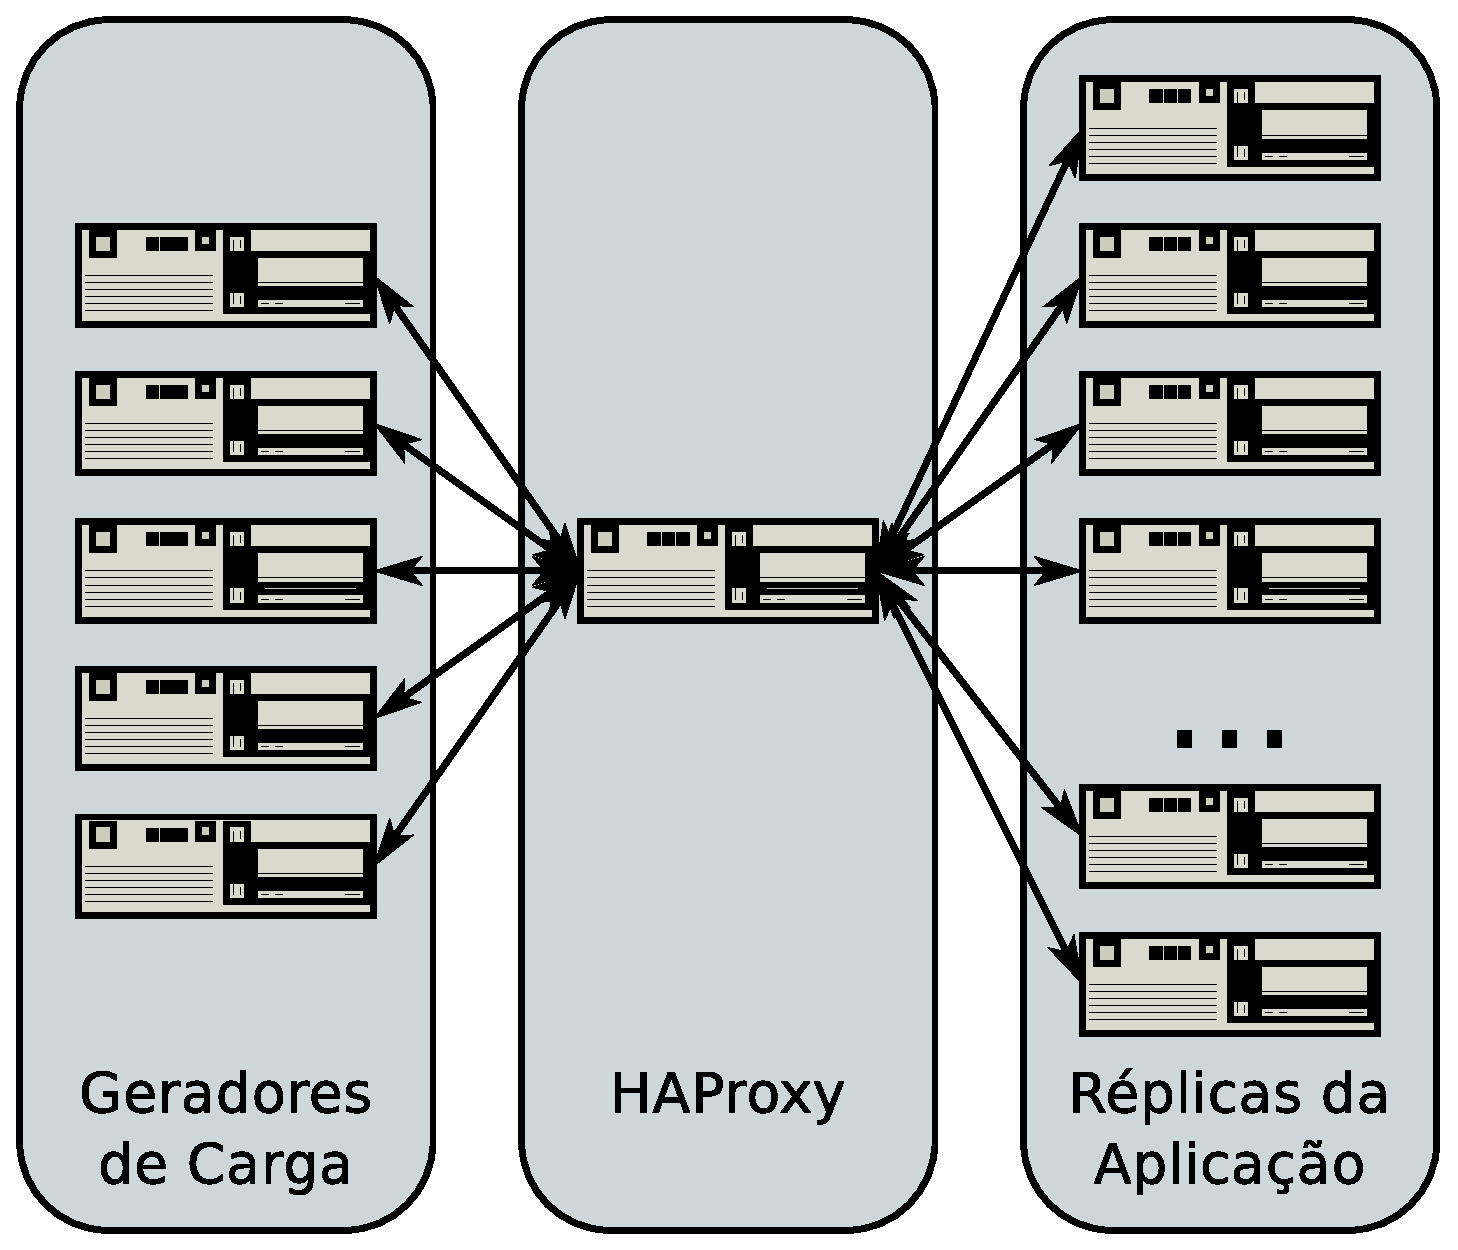
\includegraphics[width=7cm]{conteudo/capitulos/figuras/experimental-setup.dia.eps}
  \caption{Configuração experimental}
  \label{fig:setup}
\end{figure}

\subsection{Carga}\label{subsec:carga}

O gerador de carga tem como objetivo produzir a carga de trabalho requirida pelos
experimentos e coletar medidas de vazão do ponto de vista do cliente. Sendo assim, cada
instância do gerador de carga registra em \emph{log} o \emph{timestamp} de início
e fim de cada atividade, para que seja possível o computar a vazão alcançada pela
aplicação.

Os geradores de carga são processos Java que executam requisições de leitura (requisições
para o método HTTP GET) e escrita (requisições para o método HTTP PUT) respeitando um
percentual configurável para realização de cada operação. Para todos os experimentos
dedicamos 5 máquinas para atuarem como clientes, sendo que cada uma executa 1000
requisições/segundo, variando entre requisições de leitura e escrita. Esse valor é maior
do que Treplica consegue atender para essa aplicação, em todos os cenários testados. Assim
garantimos que o sistema está sempre em sua capacidade máxima. O gerador de carga
acompanha o número de requisições em aberto e limita esse número a $160$ em cada
instância, de forma a regular o fluxo de criação de requisições com o fluxo de
processamento das mesmas.

Do ponto de vista da aplicação, requisições de leitura serão atendidas localmente por uma
das réplicas, enquanto uma requisição de escrita será transformada em uma proposta e
submetida a uma rodada de consenso. Avaliando-se o custo de cada tipo de requisição,
podemos afirmar que requisições de escrita são mais caras porque envolvem mais trocas de
mensagens que requisições de leitura.

Para execução de todos os experimentos foi gerado uma carga utilizando todas as 5 máquinas
disponíveis, totalizando uma carga máxima para a aplicação de 5000 requisições/segundo,
mantida durante 300 s para cada medida experimental. Para a análise resolvemos considerar
intervalos diferentes de acordo com o cenário de teste. Tal intervalo, ao qual chamaremos
de \emph{período de análise}, será identificado em cada análise. Os experimentos foram
divididas em duas configurações, conforme mostra os dados na
\autoref{tab:configuracao_experimento}.

\begin{table}[htb]
\IBGEtab{
  \caption{Configuração da carga experimental}
  \label{tab:configuracao_experimento}
}{
  \begin{tabular}{cccc}
  \toprule
  Experimento & Requisições por segundo & Total de escrita & Total de leitura \\
  \midrule \midrule
  1           & 5000                    & 2500 (50\%)      & 2500 (50\%)      \\
  \midrule
  2           & 5000                    & 1000 (20\%)      & 4000 (80\%)      \\
  \bottomrule
\end{tabular}
}{
}
\end{table}

Identificaremos os experimentos como Experimento 1 e Experimento 2. O objetivo da
configuração do Experimento 1 é criar um cenário que exigirá bastante esforço do protocolo
Paxos devido o equilíbrio da carga de requisições de leitura e escrita. Em contra partida
a configuração do Experimento 2 proporciona um cenário com menos trocas de mensagens de
Paxos, já que a maioria das requisições (80\%) são de leitura e são atendidas localmente
em cada réplica.


\section{Experimento Transferência de Estado}\label{sec:experimento_tranferencia_estado}

A análise de desempenho para esse experimento visa responder duas questões sobre o
mecanismo de transferência de estado em Treplica:

\begin{enumerate}
  \item Qual é o desempenho do mecanismo de transferência de estado?
  \item Qual é a melhor estratégia em Treplica para recuperação de estado: transferência de
    estado ou aplicação uma a uma das instâncias de consenso?
\end{enumerate}

Para garantir a confiabilidade dos resultados decidimos variar o tamanho do estado para
medir a capacidade do mecanismo de transferência. Para criação de tais cenários,
combinamos as configurações do Experimento 1 e do Experimento 2, detalhados na
\autoref{subsec:carga}, com a adição de uma réplica leitora, conforme descrito
anteriormente. A configuração do Experimento 2 produz um estado menor devido a quantidade
de requisições de leitura. Teoricamente esse cenário é favorável para o mecanismo de
transferência de estado uma vez que a quantidade de dados trafegados pela rede é menor.

Para construção dos cenários experimentais supomos um aglomerado com cinco réplicas, todas
previamente configuradas com a aplicação de teste. Nosso objetivo é a geração da
divergência do estado replicado em uma das réplicas, para alcançar esse objetivo iniciamos
quatro réplicas simultaneamente e postergamos a inicialização de uma das réplicas.
Definimos então dois instantes no tempo:

\begin{itemize}
  \item $t1$ início da execução das requisições dos clientes;
  \item $t2$ inicialização da aplicação na quinta réplica, $t2$ acontece exatamente 180
    segundos após $t1$.
\end{itemize}

Nessa configuração, o momento $t1$ possui quatro réplicas prontas para atender as
requisições dos clientes e no momento $t2$, a quinta réplica é adicionada ao aglomerado.
Essa nova réplica, poderá ser votante ou leitora dependendo da configuração do
experimento, conforme ilustra a \autoref{fig:timeline}. Nessa versão de Treplica o
mecanismo de transferência de estado é exclusivo para replicas leitoras e vamos usar esse
fator para facilitar a comparação com o mecanismo tradicional de Treplica. Dessa forma,
ao adicionar uma réplica leitora acionamos o mecanismo de transferência de estado e ao
adicionar uma réplica votante acionamos o mecanismo de retransmissão de instância de
consenso (preenchimento de lacunas).

\begin{figure}[ht]
  \centering
  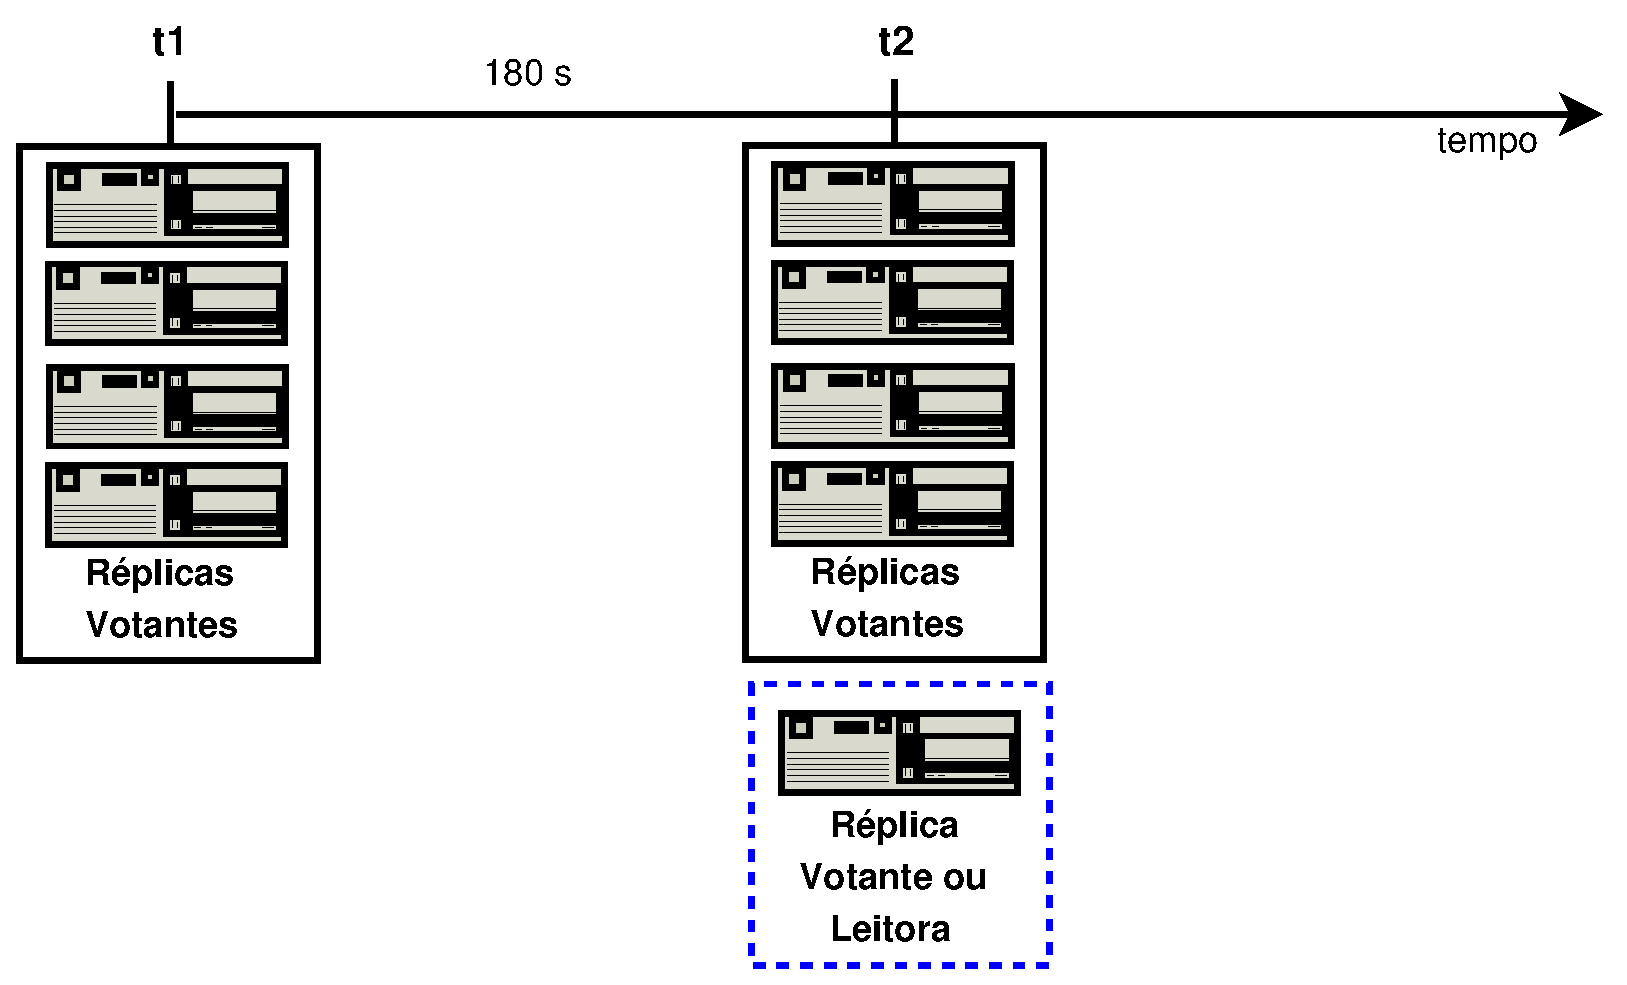
\includegraphics[width=12cm]{conteudo/capitulos/figuras/timeline.eps}
  \caption{Linha do tempo experimento transferência de estado}
  \label{fig:timeline}
\end{figure}

Nesse experimento focamos nossa análise no instante $t2$. Vamos medir e comparar o impacto
no desempenho do aglomerado causado pela adição de uma nova réplica. O foco nesse caso não
é comparação de réplicas votantes ou leitoras, mas sim os diferentes mecanismos utilizadas
por elas para receber o estado compartilhado pelo aglomerado.

Para esse experimento foram geradas requisições com uma chave aleatória e um valor de 500
bytes como na \autoref{fig:payload}. Assim, o estado crescerá proporcionalmente a
quantidade de requisições, em uma velocidade suficiente para gerar um estado da ordem de
centenas de \emph{megabytes} no tempo que o experimento executa.

\begin{figure}[ht]
  \centering
  \includegraphics[width=12cm]{conteudo/capitulos/figuras/payload.dia.eps}
  \caption{Carga associada a cada requisição de escrita}
  \label{fig:payload}
\end{figure}

\subsection{Procedimento de teste}

Os passos para execução do experimento de transferência de estado são listados a seguir:

\begin{enumerate}
  \item Iniciar manualmente o serviço do HAProxy em uma instância dedicada para o serviço
    de \emph{load balancer};
  \item Configurar, através de \emph{script}, cinco instâncias que atuarão como
    servidoras, respeitando os parâmetros que definem se a réplica atuará como votante ou
    leitora. Nesse passo é executado a instalação da JVM e Tomcat, a aplicação de teste
    foi previamente instalada Tomcat;
  \item Configurar, através de \emph{script}, cinco instâncias dedicadas para o serviço de
    cliente. Nesse passo também é instalado a JVM nas instâncias clientes e o programa de
    teste;
  \item Iniciar através de \emph{script} o serviço do Tomcat em quatro réplicas;
  \item Iniciar através de \emph{script} o programa de teste nas cinco máquinas dedicadas
    para atuarem como cliente;
  \item Aguardar 180 segundos e iniciar através de \emph{script} o serviço do Tomcat na
    quinta máquina (retardatária);
  \item Aguardar mais 180 segundos e através de \emph{script}, encerrar os processos Javas
    iniciados (cliente e servidor) e recolher os arquivos de \emph{log} dos clientes e
    servidores.
\end{enumerate}

\subsection{Resultados e Análise}

Nesta subseção responderemos as duas perguntas feitas no início dessa seção: (1) Qual é o
desempenho do mecanismo de transferência de estado? (2) Qual é a melhor estratégia em
Treplica para recuperação de estado: transferência de estado ou aplicação uma a uma das
instâncias de consenso?

Os valores das métricas foram coletados ao longo de 10 execuções e os valores apresentados
correspondem a média dessas execuções.

\subsubsection{Desempenho absoluto - Pergunta 1}

Para medir o desempenho do mecanismo de transferência de estado estabelecemos os seguintes
parâmetros para coleta e medição de desempenho:

\begin{itemize}
  \item Tempo total para envio do estado da réplica receptora para réplica doadora,
    incluindo tempo para estabelecer a conexão TCP entre as réplicas;
  \item Tamanho do estado enviado;
  \item Tempo total para ativação de uma réplica leitora. Essa medida leva em consideração
    o tempo que a réplica demorou para estar apta a processar mensagens da aplicação.
\end{itemize}

A \autoref{fig:dados_transf_estado} (a) exibe o tamanho do estado transferido pelo
Experimento 1 (50\% de requisições de leitura) e pelo Experimento 2 (80\% de requisições
de leitura). Comparando os resultados de tempo de transferência, ilustrado na
\autoref{fig:dados_transf_estado} (b), podemos afirmar que o desempenho do mecanismo de
transferência de estado está ligado diretamente com o tamanho do estado a ser transferido.
Em outras palavras, quanto maior o estado maior o tempo gasto para transferi-lo.

\begin{figure}[ht]
  \centering
  \includegraphics[width=14cm]{conteudo/capitulos/figuras/dados-transf.eps}
  \caption{Resultado transferência de estado}
  \label{fig:dados_transf_estado}
\end{figure}

Os resultados ilustrado pela \autoref{fig:dados_transf_estado} também são exibidos nas
\autoref{tab:dados_transf_estado1} (Experimento 1) e \autoref{tab:dados_transf_estado2}
(Experimento 2).

\begin{table}[htb]
\IBGEtab{
  \caption{Desempenho da transferência de estado no Experimento 1}
  \label{tab:dados_transf_estado2}
}{
  \begin{tabular}{cccc}
  \toprule
                & Tempo de Transferência & Tamanho do Estado & Tempo de Ativação \\
  \midrule \midrule
  Média         & 1.832s                 & 140.590Mb          & 2.133s            \\
  \midrule
  Mediana       & 1.867s                 & 141.535Mb          & 2.209s            \\
  \midrule
  Desvio Padrão & 0.945                  & 1.934              & 0.631             \\
  \bottomrule
\end{tabular}
}{
}
\end{table}

\begin{table}[htb]
\IBGEtab{
  \caption{Desempenho da transferência de estado no Experimento 2}
  \label{tab:dados_transf_estado1}
}{
  \begin{tabular}{cccc}
  \toprule
                & Tempo de Transferência & Tamanho do Estado & Tempo de Ativação \\
  \midrule \midrule
  Média         & 1.282s                 & 85.096Mb          & 1.533s            \\
  \midrule
  Mediana       & 1.305s                 & 85.150Mb          & 1.513s            \\
  \midrule
  Desvio Padrão & 0.079                  & 0.296             & 0.160             \\
  \bottomrule
\end{tabular}
}{
}
\end{table}

Considerando o tempo de transferência e o tamanho do estado, podemos calcular a vazão em
\emph{Megabytes}/segundo que o mecanismo de transferência de estado atingiu. Também
podemos calcular a o consumo de banda que foi utilizada por cada transferência. A
\autoref{fig:vazao_transf} ilustra esses dois cálculos, analisando os resultados podemos
verificar que o mecanismo de transferência de estado utiliza a banda disponível de forma
eficiente.

\begin{figure}[ht]
  \centering
  \includegraphics[width=14cm]{conteudo/capitulos/figuras/vazao-transf.eps}
  \caption{Vazão transferência de estado}
  \label{fig:vazao_transf}
\end{figure}

\begin{table}[htb]
\IBGEtab{
  \caption{Vazão transferência de estado}
  \label{tab:dados_vazao}
}{
  \begin{tabular}{ccc}
  \toprule
  Estado (Mb) & Vazão (Mbps) & Consumo da banda (\%)  \\
  \midrule \midrule
  140.59      & 614          & 61                     \\
  85.096M     & 531          & 53                     \\
  \bottomrule
\end{tabular}
}{
}
\end{table}

Colocar texto aqui sobre rsync!

\begin{figure}[ht]
  \centering
  \includegraphics[width=7cm]{conteudo/capitulos/figuras/dados-rsync.eps}
  \caption{Resultado transferência transferência de arquivo com rsync}
  \label{fig:dados_rsync}
\end{figure}

\begin{table}[htb]
\IBGEtab{
  \caption{Desempenho da transferência de arquivo com rsync}
  \label{tab:dados_rsync}
}{
  \begin{tabular}{ccc}
  \toprule
                & Arquivo 140.59Mb & Arquivo 85.096Mb \\
  \midrule \midrule
  Média         & 2.084s           & 1.357s            \\
  \midrule
  Mediana       & 2.081s           & 1.317s            \\
  \midrule
  Desvio Padrão & 0.012            & 0.122             \\
  \bottomrule
\end{tabular}
}{
}
\end{table}

\subsubsection{Desempenho relativo - Pergunta 2}

A segunda pergunta definida no início dessa seção é referente a escolha da melhor
estratégia de Treplica para recuperação de estado. Para respondê-la vamos comparar as
execuções do experimento da \autoref{sec:experimento_tranferencia_estado}, onde
adicionamos ao aglomerado uma nova réplica usando o mecanismo tradicional de Treplica
(réplica votante) ou o nova réplica proposta (réplica leitora). O período de análise está
concentrado ao redor do tempo $t2$. Compararemos os dois mecanismos de recuperação de
estado analisando a quantidade de operações por segundo atendidas em um espaço de 30
segundos de execução. O período de análise contém registros de 10 segundos antes da $t2$ e
20 segundos após $t2$.

Continuamos com a mesma configuração de carga definidas pelos Experimentos 1 e 2. A
\autoref{fig:transf_estado_cenario1} ilustra a vazão instantânea do experimento que
adiciona réplicas votantes e leitoras com escala de 5 segundos durante o período de
análise configurado para 30 segundos, tomada como média das 10 execuções. Assim que o
balanceador de carga detecta a presença de uma nova réplica, começa a rotear requisições
da aplicação para ela. Essa nova réplica também passa a receber mensagens do protocolo
Paxos oriundas das outras réplicas do aglomerado.

Analisando especificamente a \autoref{fig:transf_estado_cenario1} (a), podemos verificar
um vale acentuado no momento da adição da réplica votante $rv$. A transferência de estado
tradicional utilizado por $rv$, o estado é replicado instância por instância. Fica claro
que a adição de $rv$ causa uma alteração no desempenho do aglomerado que desaparece
instantes depois quando a recuperação termina.

Por outro lado, a \autoref{fig:transf_estado_cenario1} (b) ilustra o impacto da adição de
uma réplica leitora $rl$. Podemos verificar uma alteração no número de operações
suportadas quando $rl$ é adicionada. Porém, fica claro que o distúrbio causado pela
adição de uma réplica leitora é menor. Nesse caso, a replicação de estado em $rl$ acontece
através da atuação do mecanismo de transferência de estado. Ou seja, o estado é
transferido usando um mecanismo de lote mais eficiente (TCP), causando menos impacto no
desempenho do aglomerado.

\begin{figure}[ht]
  \centering
  \includegraphics[width=14cm]{conteudo/capitulos/figuras/final-transf-estado-pr50.eps}
  \caption{Desempenho da adição de uma nova réplica no Experimento 1}
  \label{fig:transf_estado_cenario1}
\end{figure}

O Experimento 2 está configurado com um maior número de requisições de leitura, a
\autoref{fig:transf_estado_cenario2} ilustra seu desempenho, forma similar a
\autoref{fig:transf_estado_cenario1}. Mais uma vez podemos observar menos impacto no
número de requisições quando adicionamos uma réplica leitora, caracterizando assim o bom
desempenho do mecanismo de transferência de estado nos dois cenários experimentais.

\begin{figure}[ht]
  \centering
  \includegraphics[width=14cm]{conteudo/capitulos/figuras/final-transf-estado-pr80.eps}
  \caption{Desempenho da adição de uma nova réplica no Experimento 2}
  \label{fig:transf_estado_cenario2}
\end{figure}

A \autoref{fig:analise_final_transf_estado} resume desempenho total do sistema ao longo do
período de análise, medido pelo número de operações por segundo atendidas e pelo tempo de
resposta dessas requisições. O efeito causado pela redução de mensagens solicitando o
envio do histórico das decisões de consenso também são benéficos quando analisamos o
desempenho das duas estratégias, conforme ilustrado na
\autoref{fig:analise_final_transf_estado} (a).

Para o Experimento 1 a proposta de transferência de estado obteve um desempenho $7.06\%$
superior (202,163 operações por segundo), enquanto que no Experimento 2 o aumento de
desempenho foi de $12.60\%$ (466 operações por segundo). Realizamos um teste-t
independente para cada uma dessas duas diferenças e o resultado produziu um valor $t$
estatisticamente significativo para o Experimento 1 ($t_{(10)}=9.74$, $p < 0.0001$) e para
o Experimento 2 ($t_{(10)}=31.15$, $p < 0.0001$).

A maior diferença entre a adição de uma réplica votante ou leitora está no tempo de
resposta do período de análise. Nesse caso estamos comparando os mecanismos de
transferência de estado configurado nas duas réplicas. No Experimento 1 o mecanismo de
transferência de estado obteve tempos de resposta $84.46\%$ menores (739.76 ms) que a
reexecução individual de operações, enquanto que no Experimento 2 a melhora foi de
$79.20\%$ (867.75 ms). Novamente, realizamos um teste-t independente para cada uma dessas
duas diferenças e o resultado produziu um valor $t$ estatisticamente significativo para o
Experimento 1 ($t_{(10)}=37.33$, $p < 0.0001$) e para o Experimento 2 ($t_{(10)}=61.93$,
$p < 0.0001$).

Analisando o resultado ilustrado na \autoref{fig:analise_final_transf_estado} (b) fica
claro, que para esses cenários de testes a melhor escolha para transferência de estado é a
utilização do mecanismo proposto por esse trabalho.

\begin{figure}[ht]
  \centering
  \includegraphics[width=14cm]{conteudo/capitulos/figuras/final-transf-estado.eps}
  \caption{Comparação do desempenho do mecanismo de transferência de estado}
  \label{fig:analise_final_transf_estado}
\end{figure}

Quando comparamos os dois experimentos, podemos verificar que o Experimento 2 consegue
suportar mais operações por segundo (\autoref{fig:analise_final_transf_estado} (a)). Isso
se deve ao fato da redução de iterações entre as réplicas requiridas por uma requisição de
leitura, predominante no Experimento 2. Os resultados ilustrado pela
\autoref{fig:analise_final_transf_estado} também são exibidos na
\autoref{tab:adicionando_replica_votante} (adicionando uma réplica votante) e na
\autoref{tab:adicionando_replica_leitora} (adicionando uma réplica leitora).

\begin{table}[htb]
\IBGEtab{
  \caption{Desempenho para incorporação de uma réplica votante}
  \label{tab:adicionando_replica_votante}
}{
  \begin{tabular}{ccccc}
  \toprule
  Leitura & Operações/segundo & Desvio Padrão & Tempo de Resposta (ms) & Desvio Padrão \\
  \midrule \midrule
  50\%    & 2862.933          & 54.491        & 875.824                & 61.181        \\
  \midrule
  80\%    & 3698.806          & 33.976        & 1095.644               & 43.157        \\
  \bottomrule
\end{tabular}
}{
}
\end{table}

\begin{table}[htb]
\IBGEtab{
  \caption{Desempenho para incorporação de uma réplica leitora}
  \label{tab:adicionando_replica_leitora}
}{
  \begin{tabular}{cccccc}
  \toprule
  Leitura & Operações/segundo & Desvio Padrão & Tempo de Resposta (ms) & Desvio Padrão \\
  \midrule \midrule
  50\%    & 3065.096          & 36.611        & 136.065                & 13.540        \\
  \midrule
  80\%    & 4164.806          & 32.920        & 227.890                & 10.049        \\
  \bottomrule
\end{tabular}
}{
}
\end{table}


\section{Experimento Réplicas Leitoras}\label{sec:experimento_replicas_leitoras}

Para validar a hipótese que réplicas leitoras podem aumentar o desempenho de um sistema
que utiliza Paxos, precisamos de uma carga de trabalho na qual uma parcela significativa
das requisições solicitadas sejam de leitura, pois essas réplicas não participam da
eleição de consenso. Para esse experimento utilizamos a aplicação descrita na
\autoref{sec:aplicacao}, fazendo uma combinação de réplicas com diferentes graus de uso de
memória persistente. Nosso objetivo aqui é medir o desempenho de um aglomerado com
réplicas votantes e leitoras, executamos cada experimento 10 vezes e os valores
apresentados correspondem a média dessas execuções.

Supomos duas formações diferentes de aglomerado para execução dos experimentos, ambas com
cinco réplicas cada: (1) cinco réplicas votantes para criação de uma base de comparação,
conforme ilustra a \autoref{fig:timeline_exp_leitora} (a); e (2) combinação de três
réplicas votantes e duas réplicas leitoras, conforme ilustra
\autoref{fig:timeline_exp_leitora} (b).

\begin{figure}[ht]
  \centering
  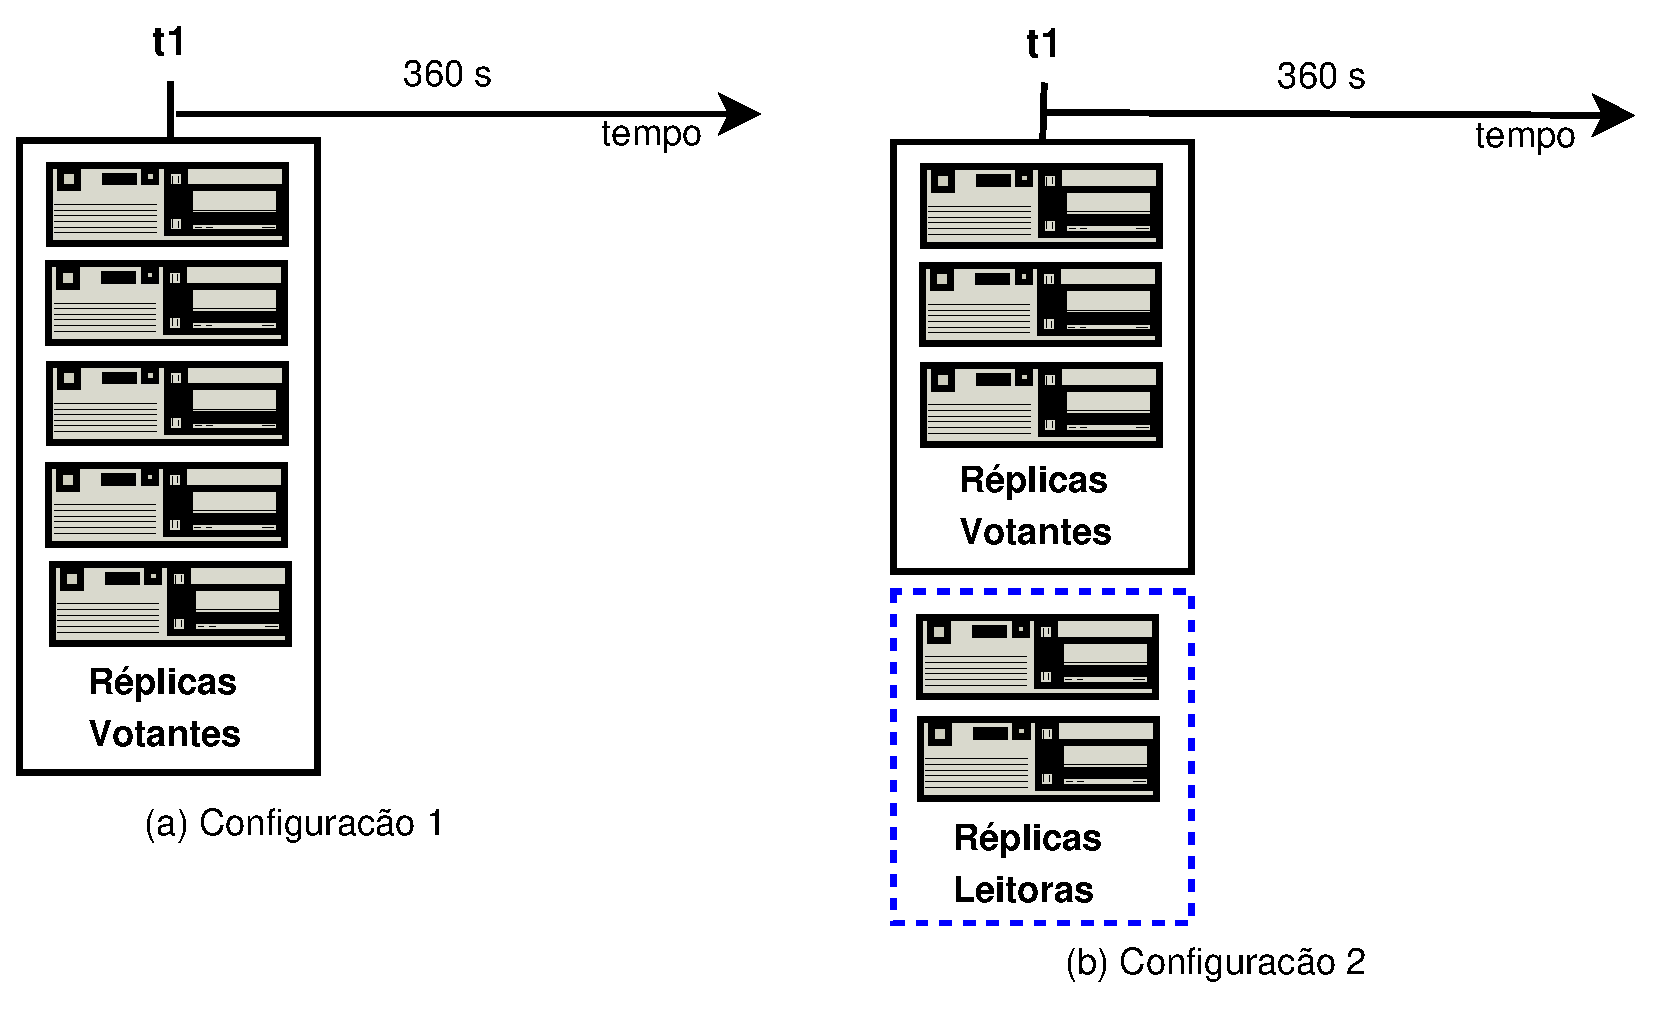
\includegraphics[width=14cm]{conteudo/capitulos/figuras/timeline_exp_leitora.eps}
  \caption{Linha do tempo experimento réplicas leitoras}
  \label{fig:timeline_exp_leitora}
\end{figure}

O tamanho do quórum para eleição do consenso durante as rodadas de Paxos depende da
formação utilizada. Na Configuração 1 não conseguimos consenso quando três réplicas falham
enquanto a Configuração 2 tolera falha em apenas duas réplicas. Podemos afirmar então que
a tolerância a falhas em Treplica está ligada diretamente como o número de réplicas
votantes existentes no aglomerado, sendo assim, a Configuração 1 é mais tolerante a
falhas.

Nesse experimento iniciamos a aplicação nas réplicas no mesmo instante de tempo para
evitar possíveis influências de outros componentes alterados em Treplica. Dessa forma, no
instante $t1$ onde se inicia a execução das requisições dos clientes, todas as réplicas
participantes do experimento já foram detectadas como ativas pelo servidor HAProxy e estão
aptas para processar requisições da aplicação.

\subsection{Procedimento de teste}\label{subsec:procedimento_teste_leitora}

Os passos para execução do experimento para medir o desempenho de réplicas leitoras são
listados a seguir:

\begin{enumerate}
  \item Iniciar manualmente o serviço do HAProxy em uma instância dedicada para o serviço
    de \emph{load balancer};
  \item Configurar, através de \emph{script}, as réplicas que atuarão como servidoras,
    respeitando a configuração de teste desejada. Nesse passo é executado a instalação da
    JVM e Tomcat, a aplicação de teste foi previamente instalada Tomcat;
  \item Configurar, através de \emph{script}, cinco instâncias dedicadas para o serviço de
    cliente. Nesse passo também é instalado a JVM nas instâncias clientes e o programa de
    teste;
  \item Iniciar através de \emph{script} o serviço do Tomcat em todas as réplicas
    servidoras;
  \item Iniciar através de \emph{script} o programa de teste nas cinco máquinas dedicadas
    para atuarem como cliente;
  \item Aguardar 360 segundos, e através de \emph{script}, encerrar os processos Javas
    iniciados (cliente e servidor) e recolher os arquivos de \emph{log} dos clientes e
    servidores.
\end{enumerate}

Aqui, diferentemente do experimento de transferência de estado, iniciamos a aplicação nas
instâncias que atuam como servidoras simultaneamente.

\subsection{Resultados e Análise}

Para análise desse experimento consideraremos as cargas do Experimento 1 e 2, que já foram
definidas na \autoref{subsec:carga}. Conforme descrito na
\autoref{subsec:procedimento_teste_leitora}, em todas as execuções desse experimento as
réplicas foram iniciadas simultaneamente. Sendo assim, eventuais sobrecargas na
inicialização de réplicas leitoras foram eliminadas pois não existe nenhum estado para ser
transferido. Em outras palavras, no momento que os geradores de carga iniciam todas as
réplicas compartilham do mesmo estado vazio.

Nesse experimento redefinimos o período de análise para 260 segundos de execução. Foram
descartamos os 20 segundos iniciais e finais visando eliminar efeitos transientes do
início e término da aplicação. A análise de desempenho para esse cenário visa responder
uma questão: Qual é o desempenho de uma réplica leitora?

Para responder essa pergunta, vamos comparar a execução das Configurações 1 e 2 no
Experimento 1 (50\% de requisições de leitura) e Experimento 2 (80\% de requisições de
leitura), executando dez vezes cada uma das quatro combinações de configuração e
experimento.

A \autoref{fig:analise_final_replica_leitora} ilustra a comparação do número médio de
requisições atendidas e tempo de resposta dessas requisições medidos no período de análise
para os dois experimentos. Fica evidente a semelhança no desempenho das duas configurações
do aglomerado nesses dois critérios.

\begin{figure}[ht]
  \centering
  \includegraphics[width=14cm]{conteudo/capitulos/figuras/final-replica-leitora.eps}
  \caption{Comparação do desempenho de aglomerados com réplicas leitoras}
  \label{fig:analise_final_replica_leitora}
\end{figure}

Para maior clareza de comparação, os resultados ilustrado pela
\autoref{fig:analise_final_replica_leitora} também são exibidos na
\autoref{tab:adicionando_replica_votante} (aglomerado configurado somente réplicas
votantes) e na \autoref{tab:adicionando_replica_leitora} (aglomerado configurado com
réplicas votantes e leitoras).

\begin{table}[htb]
\IBGEtab{
  \caption{Desempenho com réplicas leitoras}
  \label{tab:desempenho_com_replica_leitora}
}{
  \begin{tabular}{ccccc}
  \toprule
  Leitura & Operações/segundo & Desvio Padrão & Tempo de Resposta (ms) & Desvio Padrão \\
  \midrule \midrule
  50\%    & 3118.375          & 40.235        & 251.804                & 2.787         \\
  \midrule
  80\%    & 4314.798          & 14.468        & 176.524                & 0.194         \\
  \bottomrule
\end{tabular}
}{
}
\end{table}

\begin{table}[htb]
\IBGEtab{
  \caption{Desempenho sem réplicas leitoras}
  \label{tab:desempenho_sem_replica_leitora}
}{
  \begin{tabular}{ccccc}
  \toprule
  Leitura & Operações/segundo & Desvio Padrão & Tempo de Resposta (ms) & Desvio Padrão \\
  \midrule \midrule
  50\%    & 3159.908          & 35.738        & 248.718                & 2.808         \\
  \midrule
  80\%    & 4262.307          & 13.246        & 179.123                & 0.231         \\
  \bottomrule
\end{tabular}
}{
}
\end{table}

Mesmo pequena a diferença é estatisticamente significativa (p=0,002). Esse é mais uma
resultado positivo para as réplicas as leitoras que conseguem se equiparar o desempenho de
réplicas votantes e possuem uma grande vantagem: adição/remoção sem necessidade de
reconfiguração total. Essa flexibilidade no redimensionamento do aglomerado utilizando
réplicas leitoras passa a ser um diferencial a ser explorado em Treplica.

